\pdftrailerid{}
\documentclass[10pt,border=1pt]{standalone}
\usepackage[T1]{fontenc}
\usepackage{mathpazo}
\usepackage{amsmath,amssymb}
\usepackage{xcolor}
\usepackage{pgfplots}
\pgfplotsset{compat=1.18}
\usetikzlibrary{shapes.geometric,positioning,arrows.meta,calc}
\definecolor{okorange}{HTML}{E69F00}
\definecolor{oksky}{HTML}{56B4E9}
\definecolor{okgreen}{HTML}{009E73}
\definecolor{okblue}{HTML}{0072B2}
\definecolor{okverm}{HTML}{D55E00}
\definecolor{okpurple}{HTML}{CC79A7}
\colorlet{accent}{okverm}
\pgfplotsset{
  safenest/.style={
    tick label style={font=\footnotesize},
    label style={font=\small},
    title style={font=\small, align=left},
    legend style={font=\footnotesize, draw=none, fill=none, cells={anchor=west}},
    grid style={black!12, line width=0.3pt},
    axis line style={black!70, line width=0.4pt},
    tick style={black!70, line width=0.4pt},
    axis lines*=left,
  },
}
\newlength{\figwidth}
\tikzset{every node/.append style={execute at begin node={\hyphenpenalty=10000\exhyphenpenalty=10000\relax}}}
\setlength{\figwidth}{18.47cm}
\begin{document}
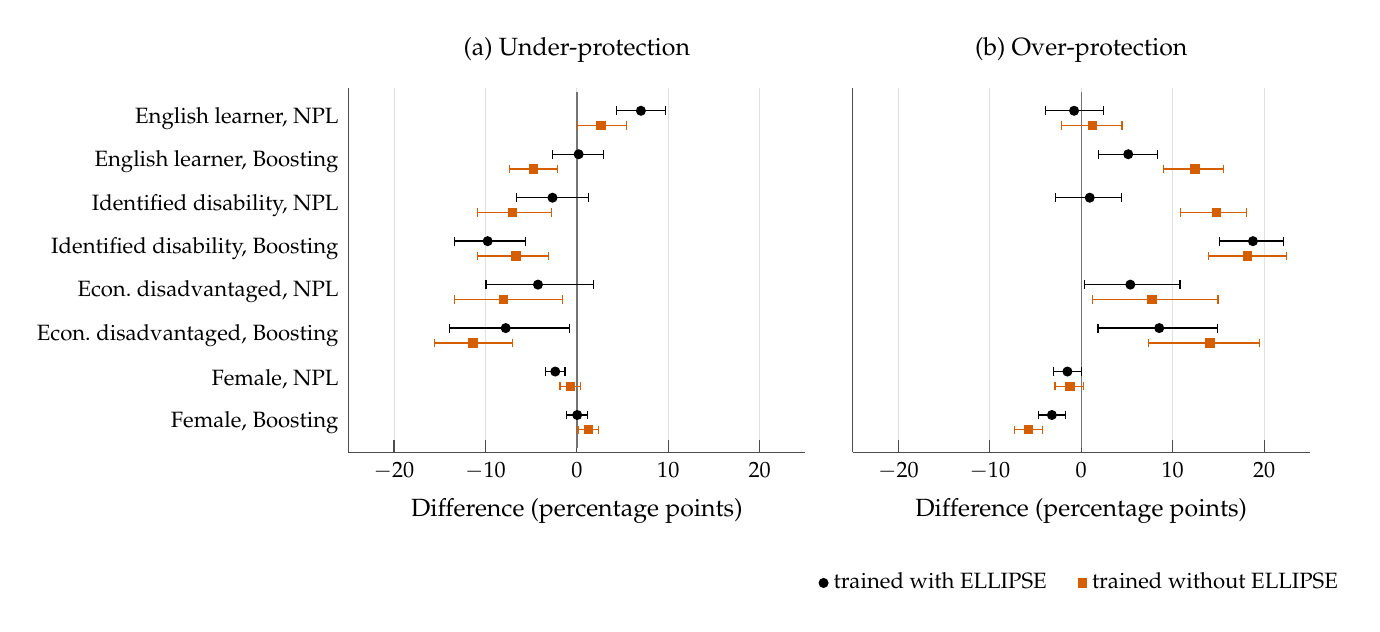
\begin{tikzpicture}
\begin{axis}[safenest, name=u, 
  width=0.40\figwidth, height=62mm, y dir=reverse,
  xmin=-25, xmax=25,
  ytick={0,...,7}, yticklabels={{English learner, NPL},{English learner, Boosting},{Identified disability, NPL},{Identified disability, Boosting},{Econ.\ disadvantaged, NPL},{Econ.\ disadvantaged, Boosting},{Female, NPL},{Female, Boosting}}, enlarge y limits=0.07,
  ytick style={draw=none},
  xmajorgrids, xlabel={Difference (percentage points)}, title={(a) Under-protection},
  legend style={at={(0.5,-0.30)}, anchor=north, legend columns=2,
                /tikz/every even column/.append style={column sep=2ex}},
]
\draw[black!55, line width=0.5pt] (axis cs:0,-0.6) -- (axis cs:0,7.6);
\addplot[only marks, mark=*, mark size=1.6pt, black,
  error bars/.cd, x dir=both, x explicit, error bar style={line width=0.5pt}]
  coordinates {(7.01,-0.17) -= (2.68,0) += (2.65,0) (0.20,0.83) -= (2.86,0) += (2.74,0) (-2.66,1.83) -= (3.93,0) += (3.93,0) (-9.75,2.83) -= (3.61,0) += (4.12,0) (-4.25,3.83) -= (5.68,0) += (6.08,0) (-7.78,4.83) -= (6.11,0) += (6.96,0) (-2.36,5.83) -= (1.06,0) += (1.07,0) (0.04,6.83) -= (1.20,0) += (1.14,0)};
\addplot[only marks, mark=square*, mark size=1.5pt, accent,
  error bars/.cd, x dir=both, x explicit, error bar style={line width=0.5pt}]
  coordinates {(2.64,0.17) -= (2.58,0) += (2.82,0) (-4.75,1.17) -= (2.59,0) += (2.63,0) (-7.02,2.17) -= (3.81,0) += (4.24,0) (-6.66,3.17) -= (4.25,0) += (3.59,0) (-8.03,4.17) -= (5.37,0) += (6.46,0) (-11.37,5.17) -= (4.23,0) += (4.35,0) (-0.69,6.17) -= (1.15,0) += (1.14,0) (1.27,7.17) -= (1.14,0) += (1.15,0)};

\end{axis}
\begin{axis}[safenest, name=o, at={($(u.east)+(6mm,0)$)}, anchor=west,
  width=0.40\figwidth, height=62mm, y dir=reverse,
  xmin=-25, xmax=25,
  ytick={0,...,7}, yticklabels={}, enlarge y limits=0.07,
  ytick style={draw=none},
  xmajorgrids, xlabel={Difference (percentage points)}, title={(b) Over-protection},
  legend style={at={(0.5,-0.30)}, anchor=north, legend columns=2,
                /tikz/every even column/.append style={column sep=2ex}},
]
\draw[black!55, line width=0.5pt] (axis cs:0,-0.6) -- (axis cs:0,7.6);
\addplot[only marks, mark=*, mark size=1.6pt, black,
  error bars/.cd, x dir=both, x explicit, error bar style={line width=0.5pt}]
  coordinates {(-0.78,-0.17) -= (3.14,0) += (3.26,0) (5.14,0.83) -= (3.21,0) += (3.24,0) (0.93,1.83) -= (3.77,0) += (3.43,0) (18.78,2.83) -= (3.69,0) += (3.32,0) (5.37,3.83) -= (4.98,0) += (5.43,0) (8.53,4.83) -= (6.70,0) += (6.35,0) (-1.51,5.83) -= (1.53,0) += (1.56,0) (-3.21,6.83) -= (1.49,0) += (1.51,0)};
\addplot[only marks, mark=square*, mark size=1.5pt, accent,
  error bars/.cd, x dir=both, x explicit, error bar style={line width=0.5pt}]
  coordinates {(1.22,0.17) -= (3.36,0) += (3.24,0) (12.42,1.17) -= (3.41,0) += (3.17,0) (14.79,2.17) -= (3.89,0) += (3.31,0) (18.18,3.17) -= (4.27,0) += (4.28,0) (7.74,4.17) -= (6.49,0) += (7.22,0) (14.08,5.17) -= (6.75,0) += (5.42,0) (-1.23,6.17) -= (1.64,0) += (1.51,0) (-5.74,7.17) -= (1.51,0) += (1.47,0)};
\legend{trained with ELLIPSE, trained without ELLIPSE}
\end{axis}\end{tikzpicture}
\end{document}
